\documentclass[11pt]{article}
\usepackage[utf8]{inputenc}
\usepackage{amsmath,amssymb,amsthm}
\usepackage{graphicx}
\usepackage{hyperref}
\usepackage{algorithm}
\usepackage{algorithmic}
\usepackage{booktabs}
\usepackage{wrapfig}

\title{ *WIP* tatbot: Tattoo Robot}
\author{Hugo Ponte}
\date{\today}

\begin{document}
\maketitle

\begin{figure}[h]
    \centering
    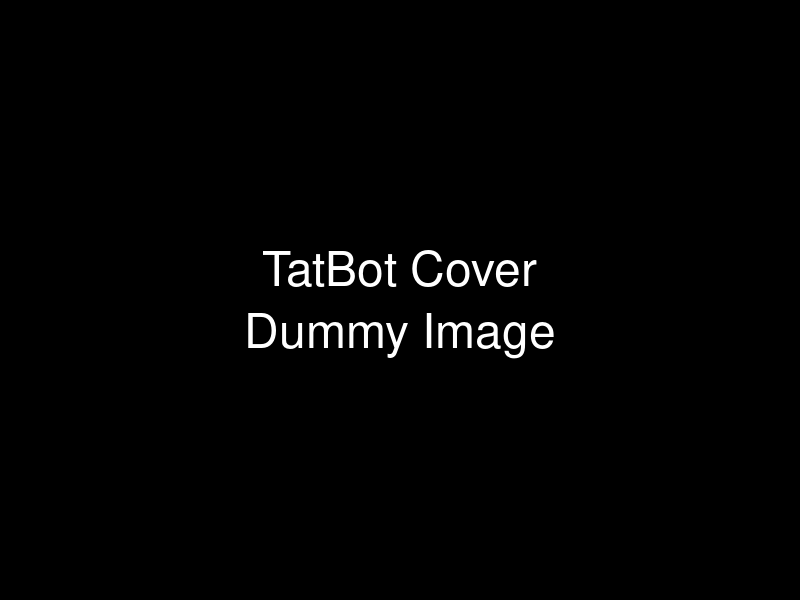
\includegraphics[width=0.8\textwidth]{figures/cover.png}
    \caption{(a) The tatbot system (hardware v0.2) (b) First human tattoo performed by the tatbot system. }
    \label{fig:cover}
\end{figure}


\begin{abstract}
*WIP* We present \textbf{tatbot}, an autonomous robotic system designed to perform tattoo artistry.
\end{abstract}

\pagebreak

\begin{figure}[h]
    \centering
    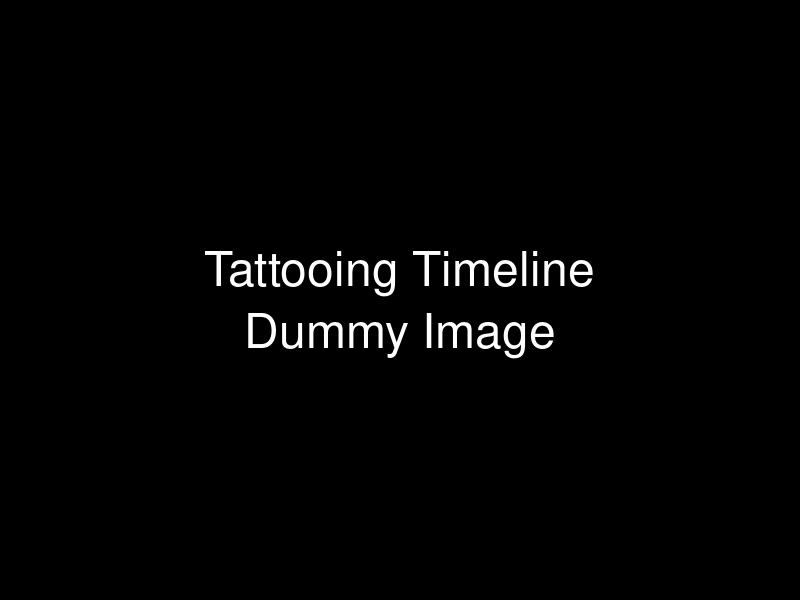
\includegraphics[width=0.8\textwidth]{figures/timeline.png}
    \caption{A history of tattoos.}
    \label{fig:timeline}
\end{figure}

\section{Background}

\subsection{History}

Tattoos are an ancient art form that predates recorded history.
Tattoos have been used as punishment, status symbols, and even therapeutic tools.
Ötzi, a frozen mummy found in the alps dated to 6272 BP, had tattoos on his arthritic joints \cite{deterwolf_worlds_oldest}.
The Yimkhiungs of Northern India perform ritualized tattooing on children as young as 5 yearls old \cite{kluger2015cultural}.
In ancient Mesopotamia, tattooing was used to mark slaves to punitively identify criminals \cite{hawken2022tattooing}.
Today tattoos have evolved and merged into a global art form that is practiced in every corner of the world.
Though some of the original symbology and purpose still remains, most modern tattoos are purely aesthetic.
In many cultures, tattoos have to be "earned". They might represent a rite of passage, family sigil, or national identy. There is still debate over cultural appropriation of tattoos.
Tattoo comes from a polynesian word \textit{tatau} which means \textit{to strike}, a reference to the traditional method of tattooing where needle penetration is achieved by striking with stick.
During the 18th and 19th centuries, the age of exploration introduced Polynesian tattoos to the west.
As a result, most modern languages now use the loanword tattoo to describe the art form over whatever traditional terminology may have existed.

\subsection{Biology}

\begin{wrapfigure}{l}{0.5\textwidth}
    \vspace{-20pt}
    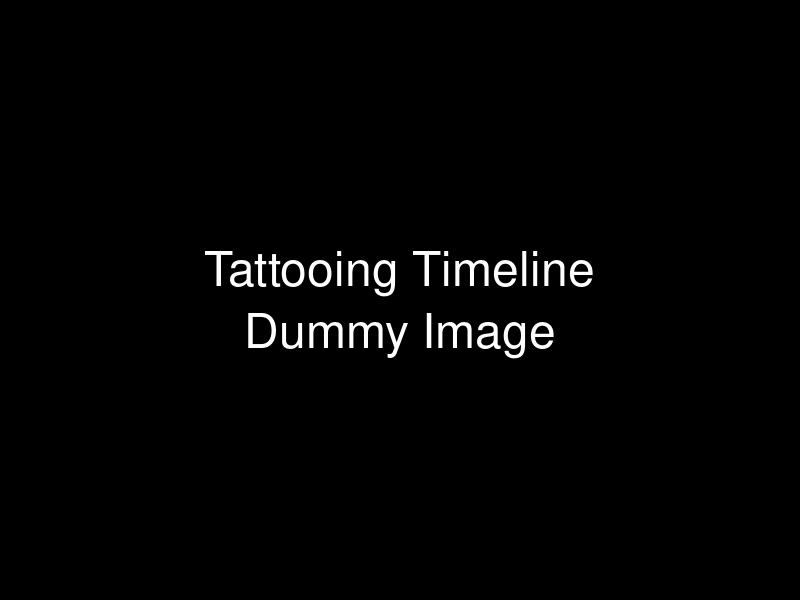
\includegraphics[width=\linewidth]{figures/timeline.png}
    \caption{A history of tattoos.}
    \label{fig:timeline_biology}
\end{wrapfigure}

The human skin is a complex organ, but it can roughly be divided into three layers:

\begin{itemize}
    \item Epidermis: outermost layer, 0.1 to 0.5mm thick, contains melanocytes, keratinocytes, and melanin.
    \item Dermis: middle layer, 1 to 4mm thick, contains blood vessels, nerves, and hair follicles.
    \item Subcutaneous tissue: innermost layer, 1 to 4mm thick, contains fat and connective tissue.
\end{itemize}

In a perfect tattoo, each needle puncture will deposit ink particles into the dermis.
Ink deposited in the epidermis will fade as the skin cells regenerate.
Ink deposited in the subcutaneous tissue will "blow out" as it diffuses outwards from the puncture site.
because tattoos penetrate the skin, they can be a vector for disease transmission.
medical grade equipment and sanitation protocols are required to prevent infection.

\begin{figure}[h]
    \centering
    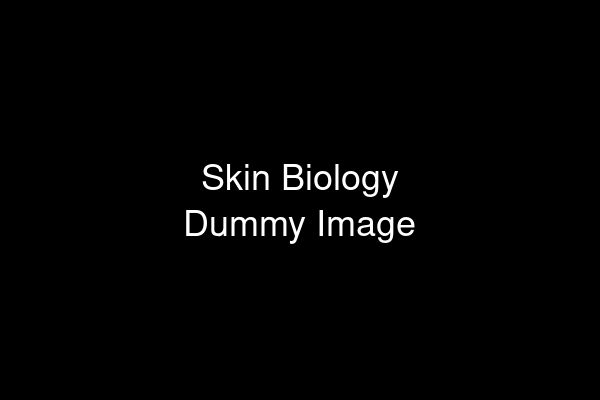
\includegraphics[width=0.8\textwidth]{figures/biology.png}
    \caption{A history of tattoos.}
    \label{fig:timeline}
\end{figure}

\pagebreak

\subsection{Technology}

Tattoo machines can be classified into two rough categories: rotary and coil.
rotary machines have become the standard for modern tattooing.
a wide variety of manufacturers compete to create the best wireless battery powered rotary machines.
voltage is modulated to control the speed of the motor, ranging from 3V to 12V.
needles are sold in pre-packaged cartridges, providing a convenient sterilized one-time use needle.
many cartridge types and vendors exist
needles are classified by their diameter, a grouping pattern, taper type, and length.
rotary machines use the rotational motion of a small electric motor to drive the up and down motion of the needle.
The distance the needle travels is called the \textit{stroke length}.

\begin{figure}[h]
    \centering
    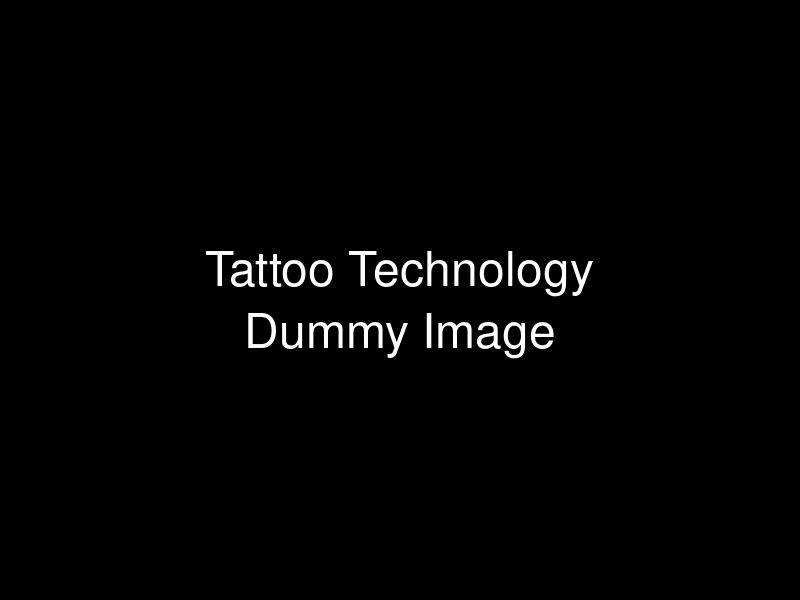
\includegraphics[width=0.8\textwidth]{figures/technology.png}
    \caption{A history of tattoos.}
    \label{fig:timeline}
\end{figure}

\subsection{Theory}

the artist controls:
\begin{itemize}
    \item the speed of the machine travel along the surface of the skin.
    \item the angle of the needle with respect to the skin surface.
    \item the depth of the needle penetration.
    \item the choice of needle cartridge.
    \item the choice of ink color (and dilution)
\end{itemize}

A tattoo $T = (m_1, m_2, \ldots, m_n)$ is a sequence of $n$ marks $m_i$.
A mark $m_i$ is pattern of ink deposition on a bounded surface $S_i$ representing a small patch of skin.
We approximate this surface using a mesh $M_i$, which is a collection of vertices $V_i$, edges $E_i$, and faces $F_i$.
Each vertex $v_j \in V_i$ has a position $p_j \in \mathbb{R}^3$.
Each edge $e_k \in E_i$ has a start vertex $s_k \in V_i$ and an end vertex $e_k \in V_i$.
Each face $f_l \in F_i$ has a normal vector $n_l \in \mathbb{R}^3$ and a center position $c_l \in \mathbb{R}^3$.
The angle of the needle with respect to the skin surface is represented by a quaternion $q_i \in \mathbb{H}$.
Each mark $m_i$ is parameterized by a start position \( \mathbf{p}_i \in \mathbb{R}^3 \), a direction vector \( \mathbf{d}_i \in \mathbb{R}^3 \), and a radius \( r_i \).
The bounded surface $S_i$ is represented by a sdf $\phi: \mathbb{R}^3 \to \mathbb{R}$.
and the skin penetration depth at a point cae computed as:
\[
d(\mathbf{x}) = -\phi(\mathbf{x}) \quad \text{(for points inside the skin)}
\]
the robot can be broken down into the arm and the tool.
in the literature the tool is also called end effector, gripper, or manipulator.
the arm is controlled in joint space $\mathbf{q} = (q_1, q_2, \ldots, q_j)$ where the number joints $J$ is $6$.
robot end effector has a position and quaternion $\mathbf{p}_{ee} \in \mathbb{R}^3 \quad \text{and} \quad \mathbf{q}_{ee} \in \mathbb{H} \quad (\text{a quaternion})$
Inverse kinematics (IK) is the process that converts the joint space coordinates \( \mathbf{q} \) into the end effector space coordinates \( (\mathbf{p}_{ee}, \mathbf{q}_{ee}) \):
\[
\text{IK}: \mathbf{q} \mapsto (\mathbf{p}_{ee}, \mathbf{q}_{ee})
\]

condition the mark on a sequence of mesh vertices
mesh transformers are probably very good for generating these kind of vertex sequences
you can then condition the arm controller on the vertex sequence

\pagebreak

\section{tatbot}

\subsection{Hardware}

TatBot uses a pair of Trossen Robotics WidowXAI arms, each providing six degrees of freedom plus a gripper. The arms are driven by dedicated controller boxes on a gigabit Ethernet network.

Perception is handled by two Intel RealSense D405 cameras---one mounted on the right arm and another mounted overhead---along with five PoE overhead cameras. An NVIDIA Jetson AGX Orin and a System76 Meerkat PC handle inference and visualization, while two Raspberry Pi 5 computers manage auxiliary tasks.

Interchangeable end effectors, including a calibration cone, a tattoo machine, and a paper towel roll, attach to the arms via locating fiducials to maintain consistent poses.

\begin{table}[h]
    \centering
    \caption{Compute and camera devices used by TatBot}
    \label{tab:hardware-devices}
    \begin{tabular}{lll}
        \toprule
        Device & Type & Notes \\
        \midrule
        Jetson AGX Orin (\texttt{ojo}) & Compute & 12-core ARM, 32GB RAM \\
        System76 Meerkat (\texttt{trossen-ai}) & Compute & Intel i5-1340P, 15GB RAM \\
        Raspberry Pi~5 $\times$2 & Compute & 4-core ARM, 8GB RAM each \\
        Intel RealSense D405 $\times$2 & Camera & Wrist and overhead mounts \\
        Amcrest PoE cameras $\times$5 & Camera & Overhead coverage \\
        \bottomrule
    \end{tabular}
\end{table}

\subsection{Software}

The TatBot system relies on a suite of open-source software packages:
\begin{itemize}
    \item \textbf{viser (v0.2.23):} Used for 3D visualization and creating interactive browser-based GUIs. Essential for visualizing robot workspaces, tattoo designs, and simulation results.
    \item \textbf{Pillow (>=9.0.0,<11.0.0):} A Python Imaging Library fork, used for image manipulation tasks, which could include processing tattoo designs or camera input.
    \item \textbf{trossen-arm (v1.8.1):} The official Python library for controlling Trossen Robotics arms, likely used for interfacing with the Aloha Solo robot arm.
    \item \textbf{pyrealsense2 (v2.55.1.6486):} Python bindings for Intel RealSense SDK, used for capturing data from RealSense depth cameras, likely for environment perception and skin surface mapping.
    \item \textbf{pyroki (git+https://github.com/chungmin99/pyroki.git@main):} A robotics library, potentially used for kinematics, trajectory planning, or other robot control functions.
    \item \textbf{jax[cuda12] (>=0.4.0,<0.5.0):} A high-performance numerical computation library, accelerated with CUDA for GPU usage. Likely used for machine learning model training and inference, and complex calculations.
    \item \textbf{jaxtyping (>=0.2.25,<1.0.0):} Type annotations for JAX, enhancing code clarity and robustness for JAX-based computations.
    \item \textbf{jaxlie (>=1.3.4,<2.0.0):} A library for Lie theory operations with a JAX backend, often used in robotics for representing and manipulating rotations and transformations.
\end{itemize}

\subsection{VLA}

Vision-Language-Action (VLA) models represent a new paradigm in robotics, enabling systems to interpret visual inputs, understand natural language instructions, and generate complex action sequences in the real world.
Recent advances such as $\pi$0 \cite{Black2024pi0}, GR00T N1 \cite{Bjorck2025gr00t}, and SmolVLA \cite{Shukor2025smolvla} have demonstrated the potential of large-scale, generalist VLA models to perform a wide range of tasks across diverse robotic platforms.
These models leverage massive datasets and transformer-based architectures to bridge the gap between perception, language, and control, paving the way for more flexible and capable autonomous agents.

\subsection{Data Recipe}

swiftsketch dataset - flux/ideogram/sdxl -> switftketch svg -> ply/mesh
meshformer dataset -

Vision Language Action (VLA) models are used to merge the semantic intelligence of large pretrained VLMs and fast robotic control performed with a Diffusion Model.
$\pi_0$ \cite{Black2024pi0}, GR00T N1 \cite{Bjorck2025gr00t}, and SmolVLA \cite{Shukor2025smolvla} have demonstrated the potential of large-scale, generalist VLA models to perform a wide range of tasks across diverse robotic platforms.


finetuned VLA with 
synthetic data generated heuristically from sim
real data from recorded tatbot sessions

huggingface for dataset management

there is a fundamental magic inside modern pretrained transformers.
The space of neural programs encoded in the weights just from human data on the internet is enormous. 
Some of these neural programs serve as useful starting points for robotic control.

\section{Results}

foo

\section{Discussion}

\subsection{Other Robotic Tattoo Systems}

Tattoos are fundamentally 3D.
They flow over the surfaces and curves of the body.
Every single previous robotic tattoo system has been constrained to the 2D plane.
Robot arms have been used before, but the control is still classical.
A set of waypoints are programmed by the human operator and the robot arm just simply executes.
Modern attempts have focused on 2D gantry systems, similar to 3D printers.
The most advanced tattoo robot to date is from an Austin based startup called Blackdot.
I have personally received a tattoo from the system and can vouch for the quality of the tattoo.
The Blackdot system breaks down 2D designs into very small black dots and then tattoos each dot individually.
However, the proccess is still fundamentally limited: the control is classical, the 2D constraint is still present.
Even the designs are not AI generated, but rather come from a library of pre-existing human designs.
These robots are not artists, they are printers.
Technology has advanced and we need to create new systems that go beyond these limitations.
AI generated designs that are 3D by nature tattooed using a robotic arm controlled by AI.
Using modern imitation learning and reinforcement learning.

foo \cite{NietoBastida2023}
foo \cite{arar2025swiftsketch}
foo \cite{carlier2020deepsvg}
foo \cite{mellor2020unsupervised}
foo \cite{ha2017neural}
foo \cite{huang2019learning}
foo \cite{kotani2019teaching}

Various tattoo robots based on modified 3D printers have been demonstrated on YouTube \cite{EmilyTheEngineer2025}, a similar system \cite{YamanDeif2021}

\subsection{Robotic Artistry}

technology can create social tensions.
photography was frowned upon by those who feared it would replace portraiture.
robotic tattooing will run into tensions with human tattoo artists.
new art mediums do not replace old art mediums, they simply expand the canvas with which humanity can express itself.

\subsection{Future Work}

As it stands, tatbot is still just a proof of concept.
The design space is limited, the accuracy is still suboptimal.
My dream is to continue to work on this project, expanding it accross the world.
Cities are the heart of tattoing, where a large population creates an endless supply of skin.

\section{Conclusion}

foo

\bibliographystyle{plain}
\bibliography{references}

\end{document} 